\documentclass[
  11pt,
  letterpaper,
   addpoints,
   answers
  ]{exam}

\usepackage{../exercise-preamble}
\usepackage{float}

\begin{document}

\noindent
\begin{minipage}{0.47\textwidth}

\includegraphics[width=\textwidth]{../fcfm_die}
\end{minipage}
\begin{minipage}{0.53\textwidth}
\begin{center} 
\large\textbf{Análisis de señales} (EL3203-2) \\
\large\textbf{Clase auxiliar 1} \\
\normalsize Prof.~ Jorge Silva.\\
\normalsize Prof.~Aux.~Erik Sáez
\end{center}
\end{minipage}

\vspace{0.5cm}
\noindent
\vspace{.85cm}

\begin{questions}
    %%%%%%%%%%%%%%%%%%%%%%%%%%%
\question Responda lo siguiente:
\begin{enumerate}

  \item Demuestre que una señal coseno discreta es periódica si y sólo si la frecuencia es racional:
  \begin{equation}
    (x[n])_{n\in\mathbb{Z}}
    =\bigl(A\cos(2\pi f\,n+\varphi)\bigr)_{n\in\mathbb{Z}}
    \quad\Longleftrightarrow\quad f\in\mathbb{Q}.
  \end{equation}

  \item Considere la siguiente familia de señales exponenciales:
  \begin{equation}
    (s_k[n])_{n\in\mathbb{Z}}
    =\left(e^{\,\mathrm{j}\frac{2\pi k}{N}\,n}\right)_{n\in\mathbb{Z}},
    \qquad k=0,1,2,\ldots
  \end{equation}
  Muestre que su período fundamental está dado por
  \begin{equation}
    N_p \;=\; \frac{N}{\gcd(k,N)},
  \end{equation}
  donde \(\gcd(\cdot,\cdot)\) denota el máximo común divisor.
\end{enumerate}
    %%%%%%%%%%%%%%%%%%%%%%%%%%%
  \begin{solution}

\subsection*{Resolución 1.1}

Demostraremos que una señal coseno discreta \(x[n] = A\cos(2\pi f\,n+\varphi)\) es periódica si y sólo si la frecuencia \(f\) es racional.

\emph{(\(\Rightarrow\)): Si \(x[n]\) es periódica, entonces \(f \in \mathbb{Q}\)}

Supongamos que \(x[n]\) es \(N\)-periódica para algún \(N \in \mathbb{Z}^+\). Entonces:
\begin{align}
x[n+N] &= x[n] \quad \forall n \in \mathbb{Z} \\
A\cos\!\big(2\pi f(n+N)+\varphi\big) &= A\cos\!\big(2\pi fn+\varphi\big)
\end{align}

Esto implica que las fases deben cumplir que el término \(2\pi fN\) debe ser un múltiplo entero de \(2\pi\) para que se cumpla la periodicidad; por tanto:
\begin{equation}
2\pi f(n+N) + \varphi = 2\pi fn + \varphi + 2\pi m
\end{equation}
para algún entero \(m\) (usando la periodicidad del coseno). Luego, simplificando:
\begin{align}
2\pi fN &= 2\pi m \\
f &= \frac{m}{N} \in \mathbb{Q}
\end{align}
Por lo tanto, si \(x[n]\) es periódica, entonces \(f\) debe ser racional.

\emph{(\(\Leftarrow\)): Si \(f \in \mathbb{Q}\), entonces \(x[n]\) es periódica}

Supongamos que \(f = \frac{k}{N}\) donde \(k, N \in \mathbb{Z}\) y \(\gcd(k,N) = 1\) (fracción en forma irreducible).

Evaluemos \(x[n+N]\):
\begin{align}
x[n+N] &= A\cos\!\Big(2\pi \frac{k}{N}(n+N)+\varphi\Big) \\
&= A\cos\!\Big(2\pi\frac{k}{N}n + 2\pi k + \varphi\Big) \\
&= A\cos\!\big(2\pi\frac{k}{N}n + \varphi\big) \quad \text{(ya que } 2\pi k \text{ es múltiplo de } 2\pi\text{)} \\
&= x[n]
\end{align}

Por lo tanto, \(x[n]\) es \(N\)-periódica. Además, como \(f = \frac{k}{N}\) está en forma irreducible, el período fundamental es exactamente \(N_0 = N\). Así, se demuestra ambas direcciones de la equivalencia:
\begin{equation}
\boxed{x[n] = A\cos(2\pi f\,n+\varphi) \text{ es periódica} \quad \Longleftrightarrow \quad f \in \mathbb{Q}}
\end{equation}

\subsection*{Resolución 1.2}

Sea la familia de señales \(s_k[n] = e^{\,\mathrm{j}\frac{2\pi k}{N}\,n}\); demostraremos que el período fundamental es \(N_p = \frac{N}{\gcd(k,N)}\), donde $\gcd(k,N)$ corresponde al máximo común divisor. Para que \(s_k[n]\) sea periódica con período \(P\), debe cumplirse:
\begin{equation}
s_k[n+P] = s_k[n] \quad \forall n \in \mathbb{Z}
\end{equation}

Sustituyendo la definición:
\begin{align}
e^{\,\mathrm{j}\frac{2\pi k}{N}(n+P)} &= e^{\,\mathrm{j}\frac{2\pi k}{N}n} \\
e^{\,\mathrm{j}\frac{2\pi k}{N}n} \cdot e^{\,\mathrm{j}\frac{2\pi k}{N}P} &= e^{\,\mathrm{j}\frac{2\pi k}{N}n}
\end{align}

Para que esto se cumpla para todo \(n\), necesitamos:
\begin{align}
e^{\,\mathrm{j}\frac{2\pi k}{N}P} &= 1 \\
\frac{2\pi k}{N}P &= 2\pi m \quad \text{para algún } m \in \mathbb{Z} \\
kP &= mN \label{eq:condicion_periodo}
\end{align}

Sea \(d = \gcd(k,N)\). Podemos escribir:
\begin{align}
k &= d \cdot k' \\
N &= d \cdot N'
\end{align}
donde \(\gcd(k', N') = 1\). Sustituyendo en la ecuación \eqref{eq:condicion_periodo}:
\begin{align}
d k' P &= m \cdot d N' \\
k' P &= m N'
\end{align}
Como \(\gcd(k', N') = 1\), recordemos que \(P\) es un valor entero. Para que esto se cumpla, \(m\) deberá ser múltiplo de \(k'\), por lo que definimos \(m=k'\cdot q\), con lo que resulta:
\begin{align}
  k' P &= k' q N' \\
  P &= q N'
\end{align}
Como buscamos el período mínimo, tendremos que \(q\) debe ser el menor valor posible, por lo que el menor valor positivo de \(P\) que satisface esta ecuación es:
\begin{equation}
P_{min} = N' = \frac{N}{d} = \frac{N}{\gcd(k,N)}
\end{equation}

\medskip
\textbf{Conclusión:} El período fundamental de la señal exponencial compleja es:
\begin{equation}
\boxed{N_p = \frac{N}{\gcd(k,N)}}
\end{equation}

\textbf{Observación:} Este resultado tiene sentido intuitivo:
\begin{itemize}
\item Si \(k = 0\), entonces \(N_p = N\) (señal constante)
\item Si \(\gcd(k,N) = 1\), entonces \(N_p = N\) (período máximo)
\item Si \(\gcd(k,N) = N\) (i.e., \(k\) es múltiplo de \(N\)), entonces \(N_p = 1\) (señal constante)
\end{itemize}

\end{solution}

    %%%%%%%%%%%%%%%%%%%%%%%%%%%
    \question Determine si las siguientes señales son periódicas. Si corresponde, especifique su período fundamental.
\begin{enumerate}
  \item \(x_a(t)=6\cos\big(9t+\tfrac{\pi}{3}\big)\).
  \item \(x[n]=6\cos\big(9n+\tfrac{\pi}{3}\big)\).
  \item \(x[n]=\cos\!\big(\tfrac{n}{8}\big)\,\cos\!\big(\tfrac{\pi n}{8}\big)\).
  \item \(x[n]=2\,e^{\,j\left(\tfrac{\pi}{7}n-3\right)}\).
  \item \(x[n]=\cos\!\big(\tfrac{\pi n}{2}\big)-\sin\!\big(\tfrac{\pi n}{8}\big)+3\cos\!\big(\tfrac{\pi n}{4}+\tfrac{\pi}{3}\big)\).
\end{enumerate}
%%%%%%%%%%%%%%%%%%%%%%%%%%%
% Asegúrate de tener en el preámbulo:
% \usepackage{amsmath,amssymb}

\begin{solution}

Recordemos que para determinar si una señal es periódica, se deben aplicar los siguientes criterios:

\begin{itemize}
\item \textbf{Señales continuas:} $x_a(t) = A\cos(\omega t + \phi)$ es siempre periódica con período $T_0 = \frac{2\pi}{\omega}$.
\item \textbf{Señales discretas:} $x[n] = A\cos(\omega n + \phi)$ es periódica si y solo si $\frac{\omega}{2\pi} \in \mathbb{Q}$.
\item \textbf{Suma de señales periódicas:} Si $x_1[n]$ tiene período $N_1$ y $x_2[n]$ tiene período $N_2$, entonces $x[n] = x_1[n] + x_2[n]$ tiene período $N_0 = \text{lcm}(N_1, N_2)$. Donde $\text{lcm}$ es el mínimo común múltiplo.
\end{itemize}
\subsection*{Resolución 2.1}

Para la señal $x_a(t) = 6\cos\!\left(9t+\tfrac{\pi}{3}\right)$, que es continua, el período fundamental se calcula como:
\begin{equation}
T_0 = \frac{2\pi}{\omega} = \frac{2\pi}{9} \text{ segundos}
\end{equation}
Es directo verificar que:
\begin{align}
x_a(t + T_0) &= 6\cos\!\left(9\left(t + \frac{2\pi}{9}\right) + \frac{\pi}{3}\right) \\
&= 6\cos\!\left(9t + 2\pi + \frac{\pi}{3}\right) \\
&= 6\cos\!\left(9t + \frac{\pi}{3}\right) = x_a(t)
\end{align}
La señal es periódica con período fundamental $\boxed{T_0 = \frac{2\pi}{9} \text{ s}}$.

\subsection*{Resolución 2.2}

Para la señal discreta $x[n] = 6\cos\!\left(9n+\tfrac{\pi}{3}\right)$, aplicamos el criterio de periodicidad: $\frac{\omega}{2\pi} \in \mathbb{Q}$. Aquí $\omega = 9$, entonces:
\begin{equation}
\frac{\omega}{2\pi} = \frac{9}{2\pi}
\end{equation}
Como $\pi$ es irracional, la fracción $\frac{9}{2\pi}$ también es irracional. Por lo tanto:
\begin{equation}
\frac{9}{2\pi} \notin \mathbb{Q}
\end{equation}
Por lo tanto, la señal $\boxed{\text{NO es periódica}}$.
\subsection*{Resolución 2.3}

Para la señal $x[n] = \cos\!\left(\tfrac{n}{8}\right)\cos\!\left(\tfrac{\pi n}{8}\right)$, utilizamos la identidad trigonométrica:
\begin{equation}
\cos(A)\cos(B) = \frac{1}{2}[\cos(A-B) + \cos(A+B)]
\end{equation}

Con $A = \frac{n}{8}$ y $B = \frac{\pi n}{8}$:
\begin{align}
A - B &= \frac{(1-\pi)n}{8} \\
A + B &= \frac{(1+\pi)n}{8}
\end{align}

Por lo tanto:
\begin{equation}
x[n] = \frac{1}{2}\left[\cos\!\left(\frac{(1-\pi)n}{8}\right) + \cos\!\left(\frac{(1+\pi)n}{8}\right)\right]
\end{equation}

Para cada término, verificamos si $\frac{\omega}{2\pi} \in \mathbb{Q}$:
\begin{align}
\text{Término 1:} \quad \frac{\omega_1}{2\pi} &= \frac{(1-\pi)/8}{2\pi} = \frac{1-\pi}{16\pi} \notin \mathbb{Q} \\
\text{Término 2:} \quad \frac{\omega_2}{2\pi} &= \frac{(1+\pi)/8}{2\pi} = \frac{1+\pi}{16\pi} \notin \mathbb{Q}
\end{align}

Como ambos términos son aperiódicos, la señal $\boxed{\text{NO es periódica}}$.

\subsection*{Resolución 2.4}

Para la señal $x[n] = 2e^{\,j(\frac{\pi}{7}n-3)}$, la reescribimos como:
\begin{equation}
x[n] = 2e^{-j3} \cdot e^{\,j\frac{\pi}{7}n}
\end{equation}

El factor $2e^{-j3}$ es constante y no afecta la periodicidad. Analizamos $e^{\,j\frac{\pi}{7}n}$. Para que sea periódica con período $N$, debe cumplirse:
\begin{equation}
e^{\,j\frac{\pi}{7}(n+N)} = e^{\,j\frac{\pi}{7}n}
\end{equation}
Esto requiere que $e^{\,j\frac{\pi N}{7}} = 1$, es decir:
\begin{align}
\frac{\pi N}{7} &= 2\pi m \quad \text{para algún } m \in \mathbb{Z} \\
N &= 14m
\end{align}

El menor valor positivo es $N_0 = 14$. Verificamos:
\begin{equation}
\frac{\omega}{2\pi} = \frac{\pi/7}{2\pi} = \frac{1}{14} \in \mathbb{Q}
\end{equation}

La señal es periódica con período fundamental $\boxed{N_0 = 14}$.

\subsection*{Resolución 2.5}

Para la señal $x[n] = \cos\!\left(\tfrac{\pi n}{2}\right) - \sin\!\left(\tfrac{\pi n}{8}\right) + 3\cos\!\left(\tfrac{\pi n}{4}+\tfrac{\pi}{3}\right)$, analizamos cada término:

\textbf{Término 1:} $\cos\!\left(\tfrac{\pi n}{2}\right)$ con $\omega_1 = \frac{\pi}{2}$
\begin{equation}
\frac{\omega_1}{2\pi} = \frac{1}{4} \in \mathbb{Q} \quad \Rightarrow \quad N_1 = 4
\end{equation}

\textbf{Término 2:} $-\sin\!\left(\tfrac{\pi n}{8}\right)$ con $\omega_2 = \frac{\pi}{8}$
\begin{equation}
\frac{\omega_2}{2\pi} = \frac{1}{16} \in \mathbb{Q} \quad \Rightarrow \quad N_2 = 16
\end{equation}

\textbf{Término 3:} $3\cos\!\left(\tfrac{\pi n}{4}+\tfrac{\pi}{3}\right)$ con $\omega_3 = \frac{\pi}{4}$
\begin{equation}
\frac{\omega_3}{2\pi} = \frac{1}{8} \in \mathbb{Q} \quad \Rightarrow \quad N_3 = 8
\end{equation}

Como todos los términos son periódicos, el período fundamental es:
\begin{equation}
N_0 = \text{lcm}(4, 16, 8) = 16
\end{equation}
La señal es periódica con período fundamental $\boxed{N_0 = 16}$. Esto se visualiza en el siguiente gráfico:
\begin{center}
  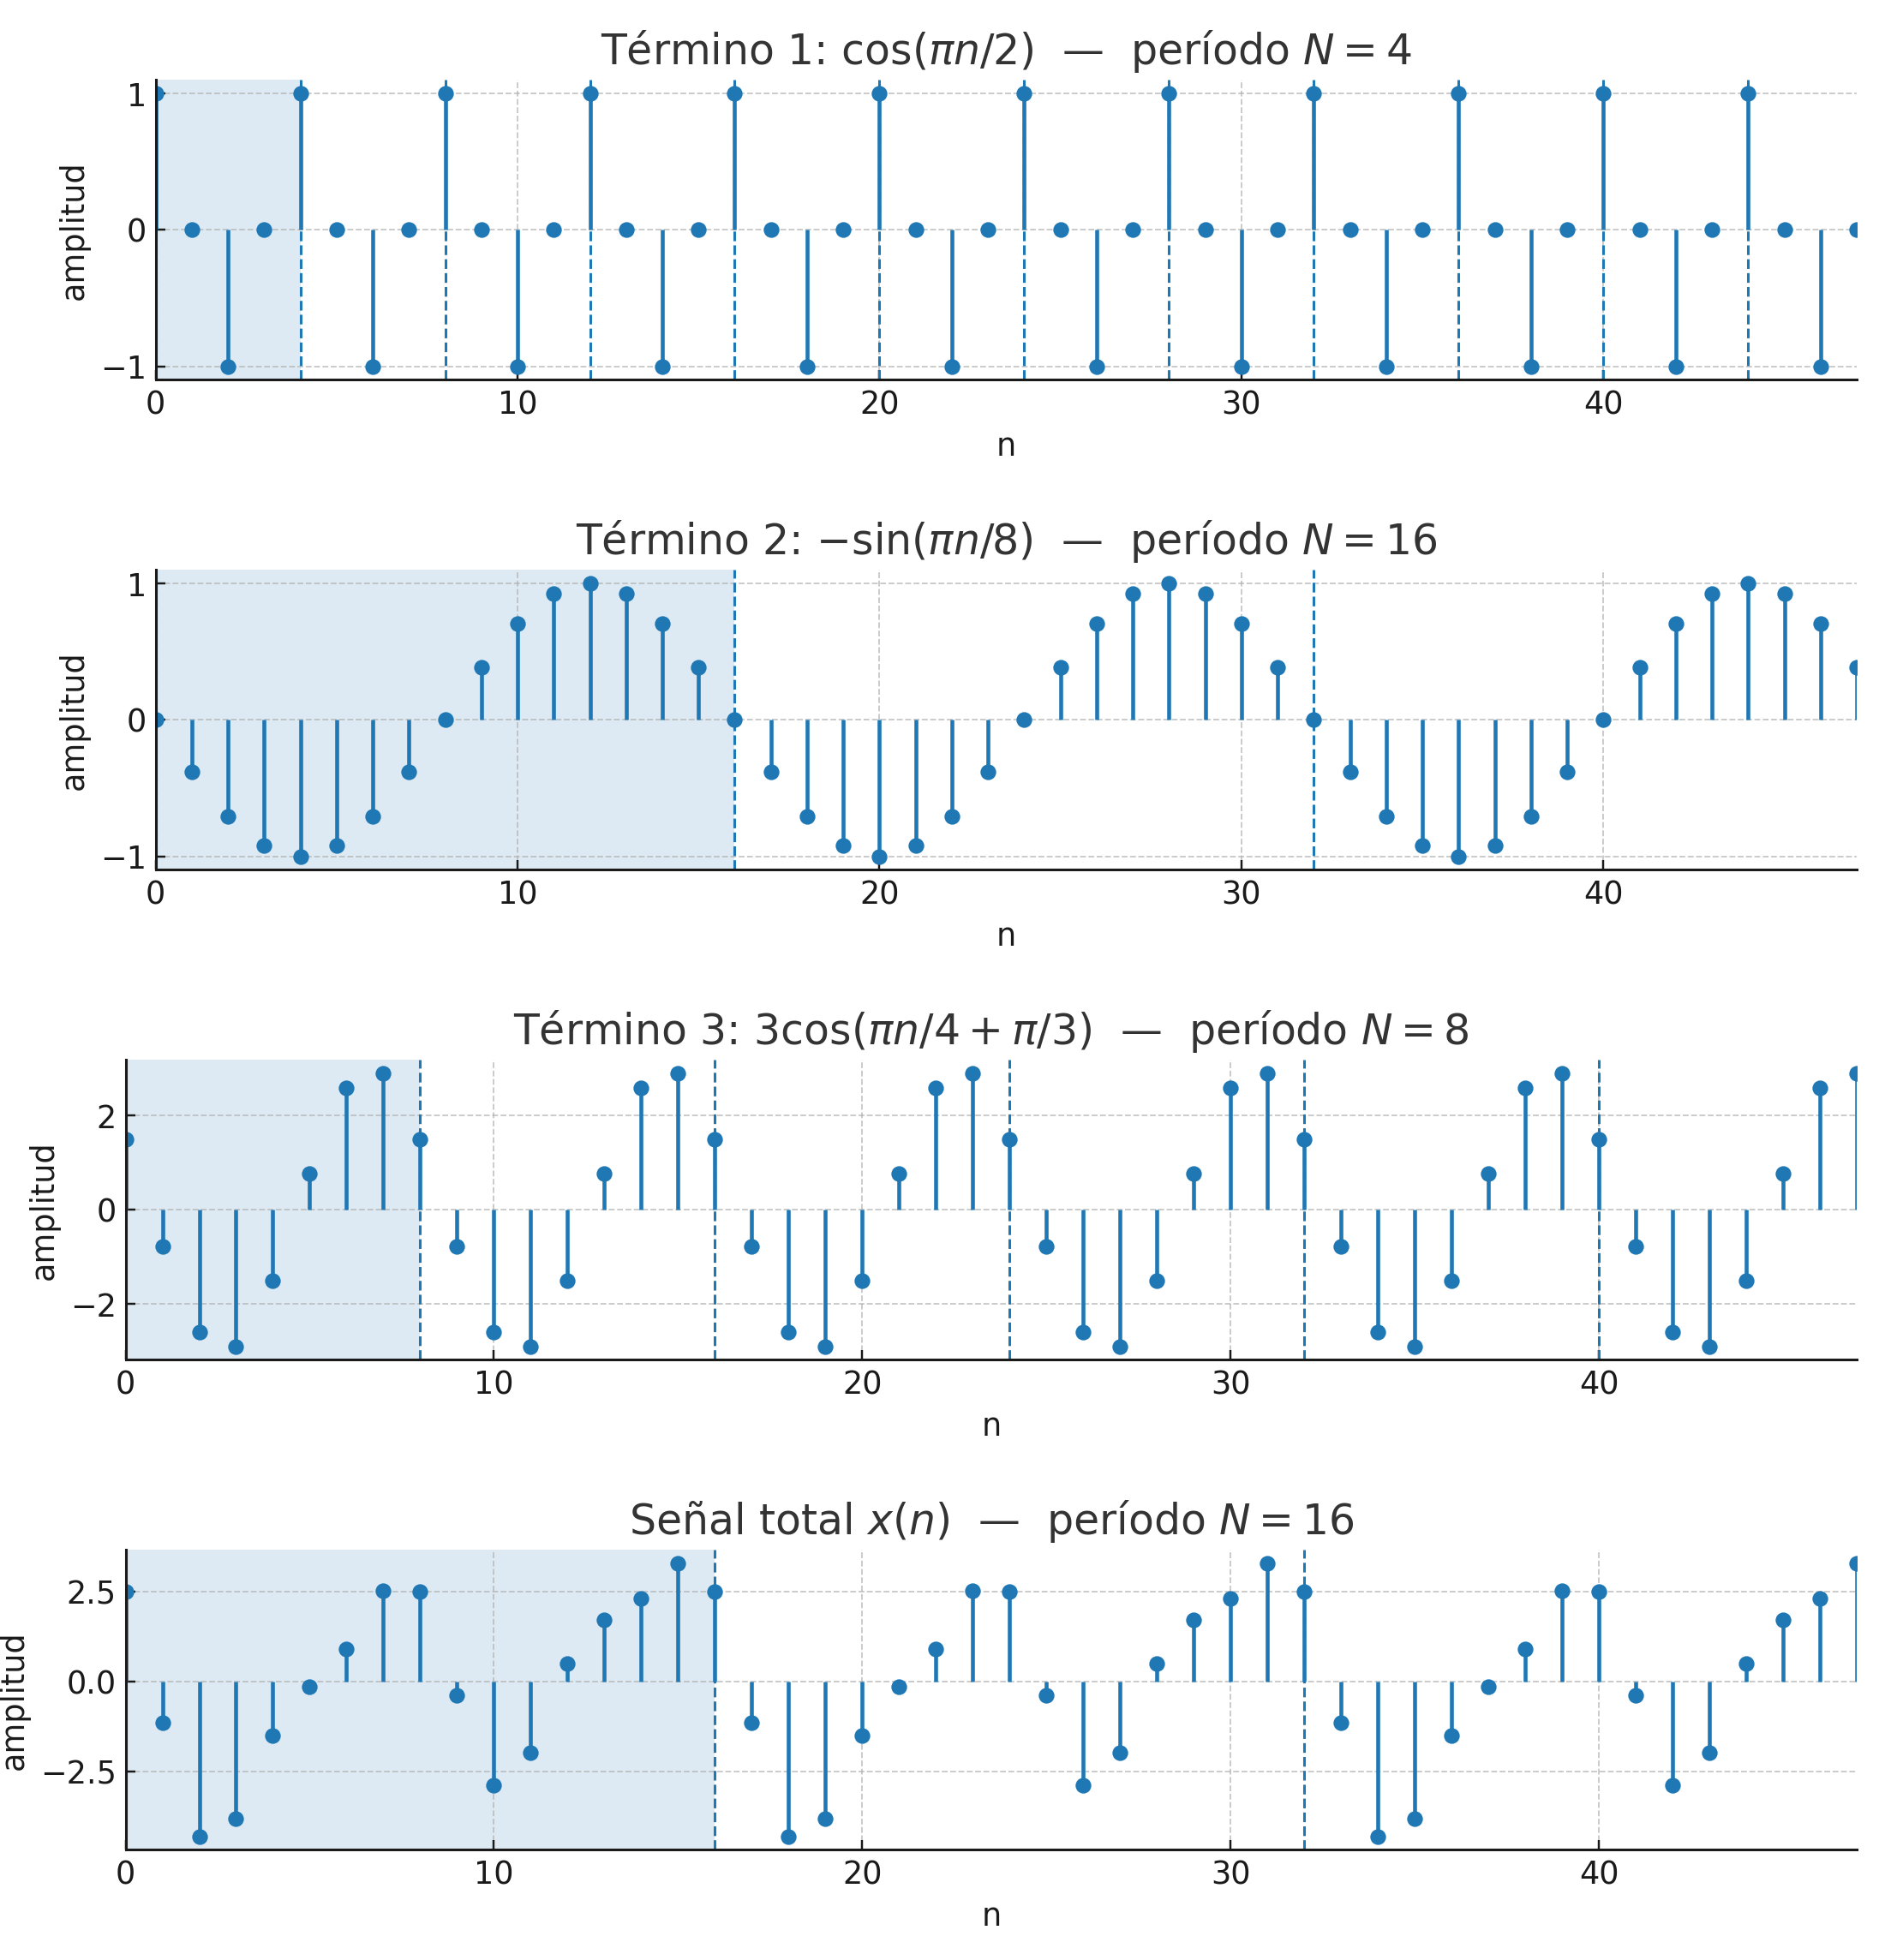
\includegraphics[width=0.8\textwidth]{Auxiliar_1_1}
\end{center}

\end{solution}

%%%%%%%%%%%%%%%%%%%%%%%%%%%
\question Considere la siguiente señal sinusoidal a tiempo continuo:
\begin{equation}
  x_a(t) \;=\; \frac{7}{2}\,\sin(200\pi\,t), 
  \qquad t \in \mathbb{R}.
\end{equation}

\begin{enumerate}
  \item Bosqueje \(x_a(t)\) para \(0 \le t \le 30\,\text{ms}\).
  \item La señal \(x_a(t)\) es muestreada a una tasa de \(F_s=300\,\text{Hz}\).
        Determine la frecuencia de la señal a tiempo discreto \(x[n]=x_a(nT_s)\),
        donde \(T_s = 1/F_s\). 
        Muestre que \(x[n]\) es periódica y determine su período fundamental.
  \item Bosqueje la señal \(x[n]\) en el mismo diagrama donde bosquejó \(x_a(t)\).
        ¿Cuál es el equivalente en milisegundos del período de \(x[n]\)?
\end{enumerate}
%%%%%%%%%%%%%%%%
% Requiere en el preámbulo:
% \usepackage{amsmath,amssymb}

\begin{solution}

\subsection*{Resolución 3.1}
La señal $x_a(t)=\frac{7}{2}\,\sin(200\pi t)$ tiene frecuencia:
\begin{equation}
\omega = 200\pi\ \text{rad/s}, \qquad f=\frac{\omega}{2\pi}=100\ \text{Hz},
\qquad T=\frac{1}{f}=0.01\ \text{s} = 10\ \text{ms}.
\end{equation}
En \(30\) ms hay \(30/10=3\) períodos completos; luego, el bosquejo de \(x_a(t)\) es:
\begin{center}
  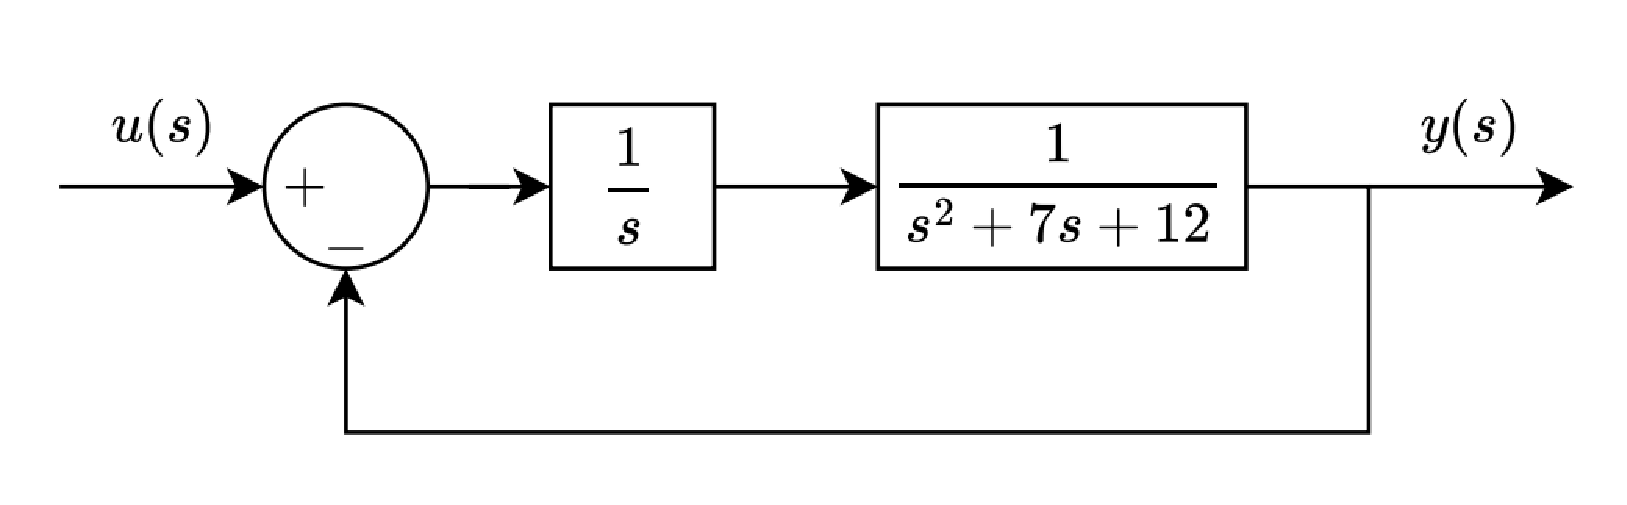
\includegraphics[width=0.7\textwidth]{Auxiliar_1_2}
\end{center}
\subsection*{Resolución 3.2}
Al muestrear con \(F_s=300\) Hz, donde \(T_s=1/F_s\), se obtiene:
\begin{align}
x[n] &= x_a(nT_s)
  =\frac{7}{2}\,\sin\!\big(200\pi\,nT_s\big)
  =\frac{7}{2}\,\sin\!\left(200\pi\,\frac{n}{300}\right) 
  = \frac{7}{2}\,\sin\!\left(\frac{2\pi}{3}\,n\right)
\end{align}
\begin{align}
  \quad\Rightarrow\quad
  \omega_d=\frac{2\pi}{3}\ \text{rad/muestra},\ \ 
  f_d=\frac{\omega_d}{2\pi}=\frac{1}{3}\ \text{ciclos/muestra}.
\end{align}
Como \(f_d=\tfrac{1}{3}\in\mathbb{Q}\), \(x[n]\) es periódica y su período fundamental es
\begin{equation}
N_0=3.
\end{equation}
El muestreo se visualiza en el siguiente gráfico:
\begin{center}
  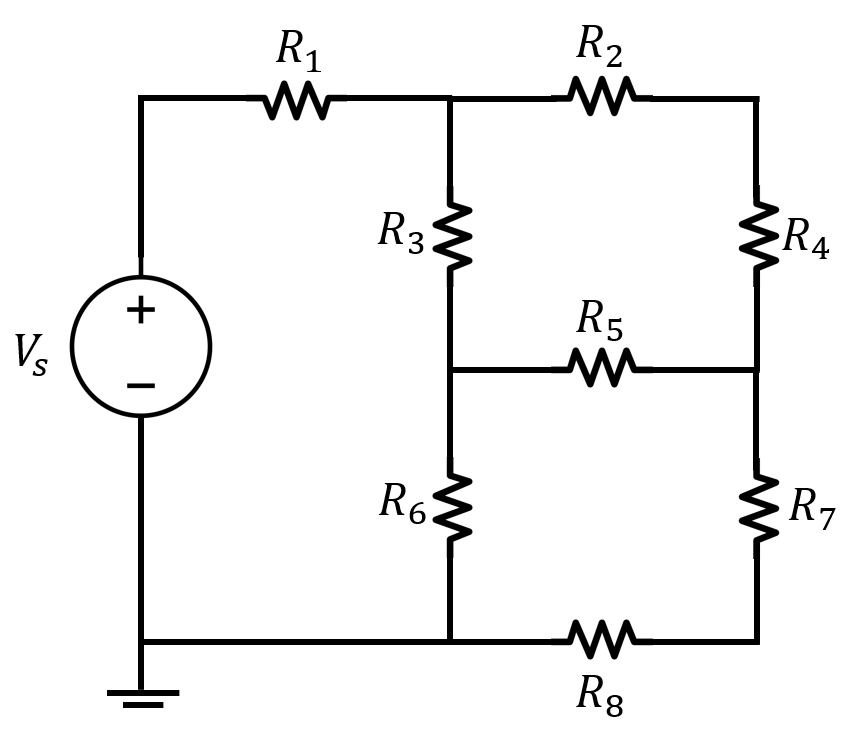
\includegraphics[width=0.7\textwidth]{Auxiliar_1_3}
\end{center}
\subsection*{Resolución 3.3}
El período de \(x[n]\) en segundos es
\begin{equation}
T_{\!x}=N_0\,T_s=3\cdot\frac{1}{300}=0.01\ \text{s}=10\ \text{ms}.
\end{equation}
Coincide con el período de la señal continua \(x_a(t)\), y gráficamente se observa que ambos períodos son iguales.
\begin{center}
  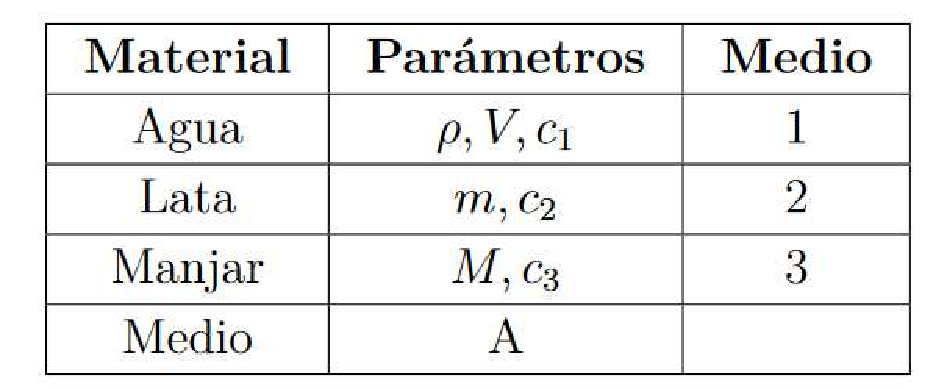
\includegraphics[width=0.7\textwidth]{Auxiliar_1_4}
\end{center}


\end{solution}

%%%%
\question Considere una señal continua \(x_a(t)\) periódica con período fundamental \(T_a\) (en segundos).

\begin{enumerate}
  \item Si se muestrea la señal \(x_a(t)\) a una tasa constante de \(F_s\) muestras por segundo, es decir, se induce la señal discreta
  \begin{equation}
    x[n] \;=\; x_a\!\left(\frac{n}{F_s}\right), \qquad \forall\, n\in\mathbb{Z},
  \end{equation}
  encuentre la(s) condición(es) que garantice(n) que \(x[n]\) sea periódica y, con ello, determine su período fundamental.

  \item Con base en el punto anterior, justifique la siguiente afirmación:
  si \(x[n]\) es periódica, entonces su período fundamental (equivalente en \textbf{segundos}) es un múltiplo de \(T_a\).
\end{enumerate}

%%%%%%%%%%%%%%%%
\begin{solution}

\subsection*{Resolución 4.1}

Dada una señal continua $x_a(t)$ periódica con período fundamental $T_a$, al muestrearla obtenemos:
\begin{equation}
x[n] = x_a\!\left(\frac{n}{F_s}\right)
\end{equation}

Para que $x[n]$ sea periódica con período $N$, debe cumplirse:
\begin{equation}
x[n+N] = x[n] \quad \forall n \in \mathbb{Z}
\end{equation}

Sustituyendo la definición de $x[n]$:
\begin{align}
x[n+N] &= x_a\!\left(\frac{n+N}{F_s}\right) \\
&= x_a\!\left(\frac{n}{F_s} + \frac{N}{F_s}\right)
\end{align}

Para que esto sea igual a $x[n] = x_a\!\left(\frac{n}{F_s}\right)$, y dado que $x_a(t)$ es periódica con período $T_a$, necesitamos que:
\begin{equation}
\frac{N}{F_s} = mT_a \quad \text{para algún } m \in \mathbb{Z}^+
\end{equation}

Esto da como resultado:
\begin{equation}
N = mF_sT_a
\end{equation}
Para que $x[n]$ sea periódica, $N$ debe ser un entero positivo, por lo tanto:
\begin{equation}
\boxed{F_sT_a \in \mathbb{Q}}
\end{equation}

Sea $F_sT_a = \frac{P}{Q}$ donde $P, Q \in \mathbb{Z}^+$ y $\gcd(P,Q) = 1$ (fracción irreducible).

Entonces $N = m\frac{P}{Q}$. Para que $N$ sea entero, $m$ debe ser múltiplo de $Q$. El menor valor positivo es $m = Q$, que da:
\begin{equation}
\boxed{N_0 = Q \cdot \frac{P}{Q} = P}
\end{equation}
Si $F_sT_a = \frac{P}{Q}$ (irreducible), entonces $N_0 = P$.

\subsection*{Resolución 4.2}

El período de $x[n]$ en segundos es:
\begin{equation}
T_x = \frac{N_0}{F_s}
\end{equation}

Sustituyendo $N_0 = P$ y usando que $F_sT_a = \frac{P}{Q}$, obtenemos $F_s = \frac{P}{QT_a}$:
\begin{equation}
T_x = \frac{P}{\frac{P}{QT_a}} = \frac{P \cdot QT_a}{P} = QT_a
\end{equation}

Como $Q \in \mathbb{Z}^+$, tenemos que:
\begin{equation}
\boxed{T_x = QT_a}
\end{equation}

Por lo tanto, el período fundamental de $x[n]$ en segundos es siempre un múltiplo entero positivo del período fundamental $T_a$ de la señal continua original. Esto significa que la señal muestreada puede tener un período temporal igual o mayor que la señal continua original, pero nunca menor. El factor $Q$ depende de la relación entre la frecuencia de muestreo y la frecuencia de la señal.

\end{solution}

\end{questions}
\end{document}